\section{Experiment 4: Light Bulbs}
\subsection{Procedure}

We observe the spectra of a compact fluorescent and an incandescent light bulb. We expect the different mechanisms of the bulbs to result in different spectral patterns. Due to time constraints in the lab, we report only qualitative findings.

\subsection{Observations}

For the CFL bulb, we observe numerous bright spectral features, particularly the bright red, green, and blue lines, and notice an overall smearing of the spectrum. These features are consistent with a mercury vapor CFL.

We repeat this setup for the incandescent light and observe a smooth spectrum of colors. The hot filament produces a continuous thermal spectrum across the visible range. Red and green appear strongest, and the violet end fades more quickly than the red.

\begin{figure}[H]
\centering
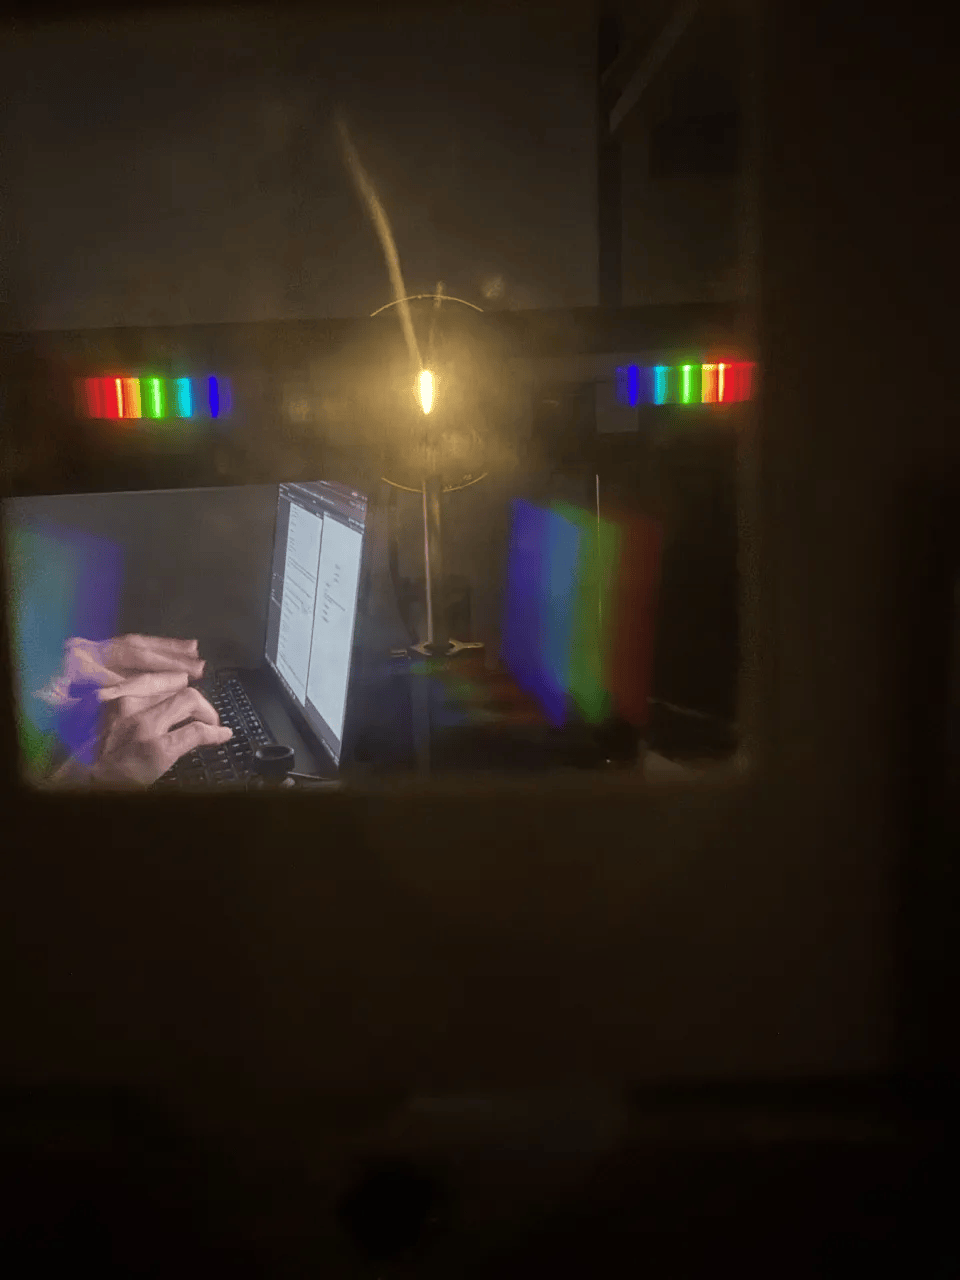
\includegraphics[width=\linewidth,trim=80bp 750bp 80bp 250bp,clip]{Photos/5CL_5_4a.png}
\caption{CFL spectrum with bright lines and overall smearing.}
\end{figure}

\begin{figure}[H]
\centering
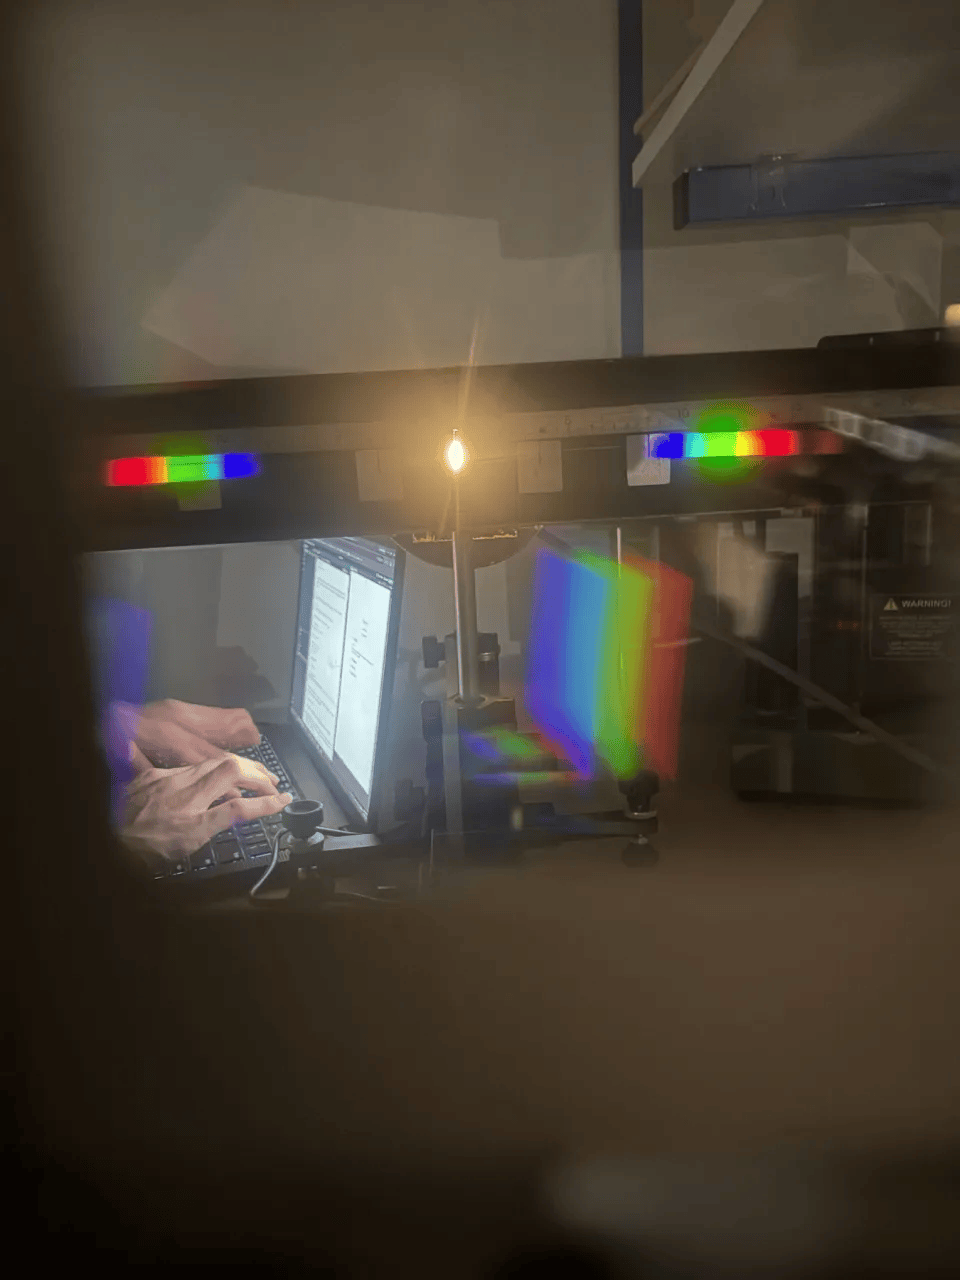
\includegraphics[width=\linewidth,trim=80bp 700bp 80bp 300bp,clip]{Photos/5CL_5_4b.png}
\caption{The smoother spectrum of the incandescent bulb.}
\end{figure}
